%	현대물리실험 보고서
%	실험3
%	202100973 이승엽

%----------------------------------------------------------------------------------------
%	PACKAGES AND DOCUMENT CONFIGURATIONS
%----------------------------------------------------------------------------------------

\documentclass[a4paper, 10pt, nanum]{CSUniSchoolLabReport}
% use UTF8 encoding
\usepackage[utf8]{inputenc}
% use KoTeX package for Korean
\usepackage{kotex}
% use ams' math font
\usepackage{amsmath}
\usepackage{hyperref}
% use table
\usepackage{graphicx}
\usepackage{multirow}
\usepackage{indentfirst}
\usepackage{setspace}
\usepackage{enumitem}
\usepackage{wrapfig}
\usepackage{epstopdf}
% use captions
\usepackage{caption}
\usepackage{subcaption}
\usepackage{blindtext}
% use layout frame
\usepackage{showframe}

% only for show page layout
\renewcommand\ShowFrameLinethickness{0.25pt}
\renewcommand*\ShowFrameColor{\color{red}}

\setlength{\parindent}{0.2in} % 들여쓰기 길이 설정
\setlength{\parskip}{3mm} % 문단 간의 간격 조절
\setstretch{1.5} % 줄간격
% \graphicpath{{Figures/}} % fig 경로 설정

\addbibresource{reference.bib} % Bibliography file (located in the same folder as the template)

%----------------------------------------------------------------------------------------
%	REPORT INFORMATION
%----------------------------------------------------------------------------------------

\title{현대물리실험 실험3 보고서 \\ Franck-Hertz experiment with neon} % Report title

\author{\textsc{Department of Physics} 202100973 이승엽}

\date{\today}

%----------------------------------------------------------------------------------------

\begin{document}

\maketitle % Insert the title, author and date using the information specified above

\begin{center}
	\begin{tabular}{l r}
		Date Performed: & May 2, 2023 \\ % Date the experiment was performed
		& May 9, 2023 \\
		Partners: & 202100969 이규리 \\ % Partner names
		& 202100989 한누리 \\
		Instructor: & Professor 이기주 \\ % Instructor/supervisor
		Typesetting: & LaTeX \\
		Datafitting: & Python \\
	\end{tabular}
\end{center}

%----------------------------------------------------------------------------------------
%	ABSTRACT
%----------------------------------------------------------------------------------------

\maketitle
% \begin{abstract}
% 	This report ...
% \end{abstract}

%----------------------------------------------------------------------------------------
%	INTRODUCTION
%----------------------------------------------------------------------------------------

\section{Introduction}

  To record a Franck-Hertz curve for neon. To measure the discontinuous energy emission of free electrons for inelastic collision. To interpret the measurement results as representing discrete energy absorption by neon atoms. To observe the Ne-spectral lines resulting from the electron-collision excitation of neon atoms. To identify the luminance phenomenon as layers with a high probability of excitation. 

%----------------------------------------------------------------------------------------
%	THEORY
%----------------------------------------------------------------------------------------

\section{Theory}

	\begin{figure}[htb!]
		\centering
		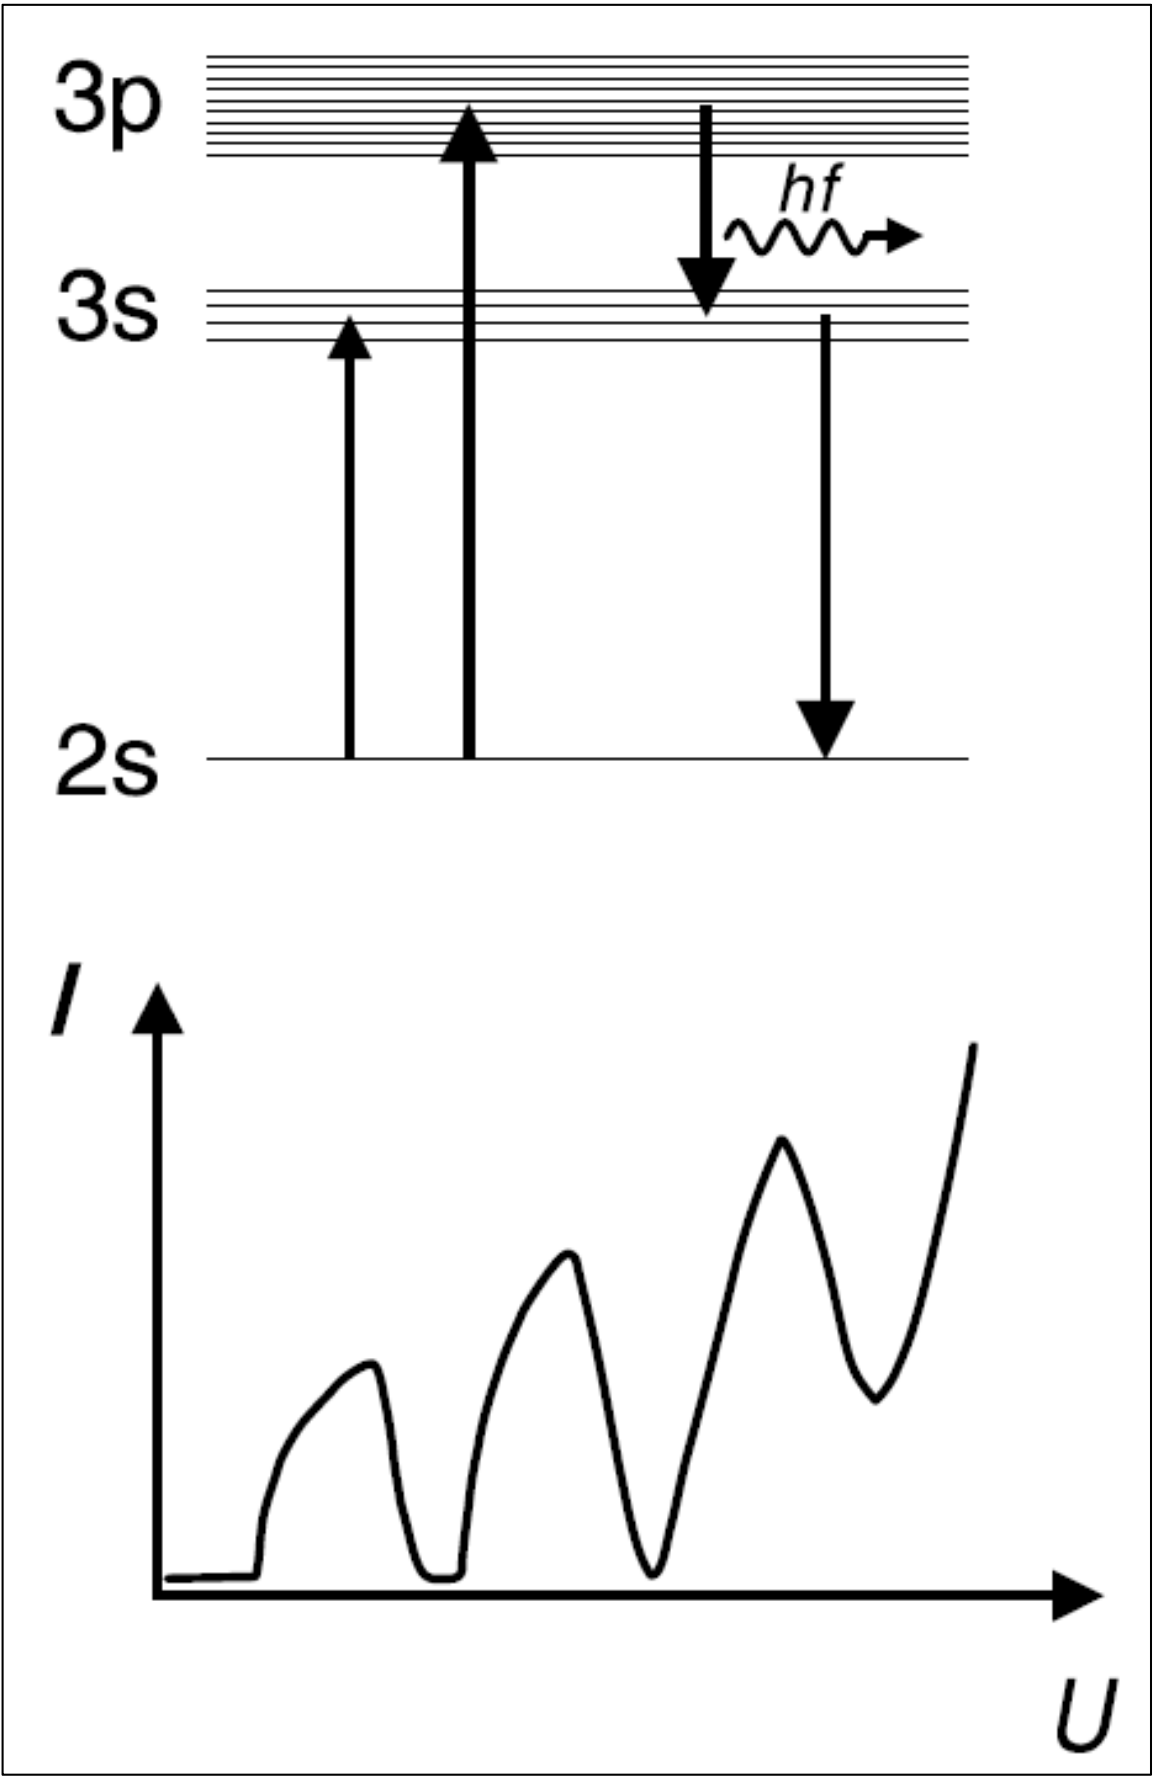
\includegraphics[width=5cm]{fig1.png}
		\caption{Top : Simplified term diagram for neon.\\ Bottom : the electron current flowing to the collector as a function of the acceleration voltage in the Franck-Hertz	experiment with neon.}
		\label{fig:1}
	\end{figure}

  J. Frank와 G. Hertz가 1914년 이후 원자의 공명 퍼텐셜을 구하기 위해 실시한 실험으로서, 수은이 네온으로 대체된 것만 빼면 같은 실험으로 당시 보어의 수소 원자 모형이 가진 전자의 Life time 문제를 설명하는 에너지 준위의 양자화를 직접적으로 보여준 실험이다. 이 실험으로 같은 해에 제창된 N.H.D. 보어의 원자 구조론에 대하여 실험적 근거를 밝혀 양자론 발전에 기여하였다. 열전자를 가속하여 전자빔을 만들어 저
  압 기체 속을 지나가게 하여 그 원자와 충돌시키도록 한자. 이 전자흐름에 의한 전류의 세기를 조사하면 전자가 원자와의 충돌에 의해 어떤 에너지의 변화를 받는가를 알 수 있다. 실험결과 , 가속 전압이 점차로 증가하여 어느 한계에 도달하면 전류가 급격히 감소
  하고, 가속 전압이 증가하면 전류는 다시 증가하여 전압이 제2차 한계 값에 이르면 다시 급속히 감소하고, 이후에는 이와 같은 전류의 극대 값이 반복된다. 이와 같이, 네온 원자에 속박된 전자의 에너지 준위가 양자화 된 것을 확인함을 목적으로 한다.

%----------------------------------------------------------------------------------------
%	EXPERIMENTAL METHOD
%----------------------------------------------------------------------------------------

\section{Experimental Method}

	\begin{figure}[htb!]
		\centering
		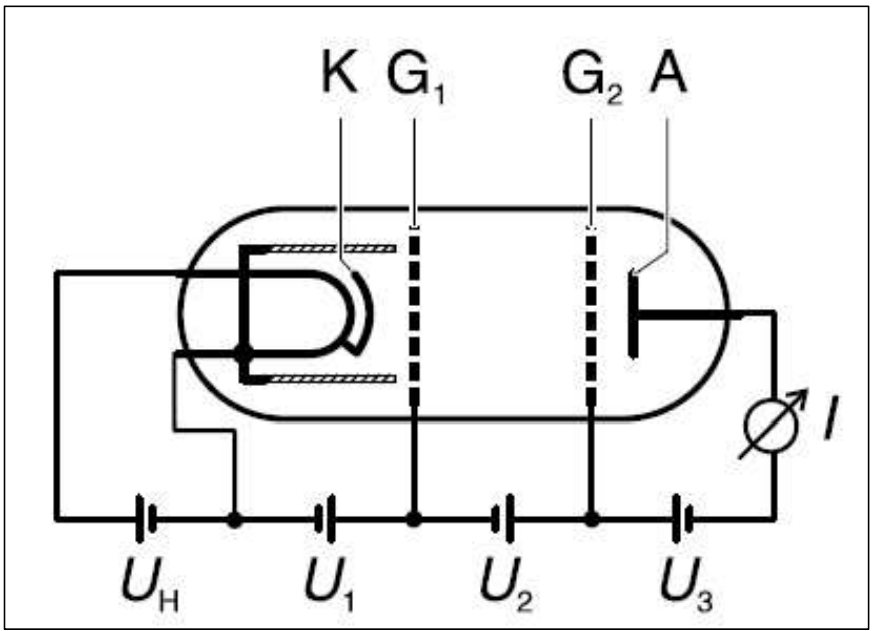
\includegraphics[width=5cm]{fig2.png}
		\caption{Schematic diagram of the Franck-Hertz tube, Ne.}
		\label{fig:2}
	\end{figure}

	Fig. 2는 실험 시 사용하는 기기의 원리를 이해하기 쉽도록 만든 회로도이다. 진공관 안에는 네온 가스가 채워져 있고, K는 음극, A는 양극, G는 grid 이다. (grid에는 가속 전압이 걸린다)

	K의 옆에 있는 필라멘트를 가열하면 K에서 방출 된 열전자는 G$_2$에 의해 가속되어 운동에너지가 증가하게 된다. 이 음전하를 띈 열전자가 G$_2$를 통과한 후 양극인 A에 걸린 역전압 $V_0$에 의해 약간 감속이 되며 A에 흡수된다. (G$_2$에 걸리는 가속전압을 증가시키면 더 많은 열전자가 A에 도달하여 플레이트 전류는 증가한다)

	진공관 속에 들어있는 네온 원자는 ground state로부터 띄엄띄엄한 에너지준위를 갖고 있기 때문에 연속적으로 분포한 아무 값의 에너지나 흡수하여 excited state로 올라가지 않는다. 보어 수소원자 모델에서 설명한 대로 에너지 준위의 차이에 해당하는 양만큼의 에너지가 공급이 되어야만 그 에너지를 흡수하여 excited state로 올라가게 된다. G$_2$의 가속전압을 서서히 올려주어 G$_2$ 주위에서의 운동에너지가 마침내 원자의 첫 번째 excited state로 올라갔을 때 그 지점에서 전자는 에너지를 잃고 멈추게 될 것이다. 따라서 이 때 전자는 A에 닿을 수 없고, 전류계의 눈금은 급격하게 줄어들게 된다. 전자가 운동에너지를 잃어버리면 그 잃어버린 에너지는 원자에 흡수된다. 이는 비탄성 충돌이며, 위의 경우 전류계의눈금이 줄기 전까지 일어나는 충돌이 바로 비탄성 충돌이다(전류계의 눈금이 줄어드는 부분은 완전 비탄성 충돌이 일어나는 순간이다).

	이 상태에서 전압을 증가시키면 또다시 일정 간격 이후 전류계의 눈금이 줄어드는 부분이 발견이 되며, 이런 식으로 세 번째, 네 번째 등등의 에너지준위와 그 간격을 알 수 있다.

	\begin{figure}[htb!]
		\centering
		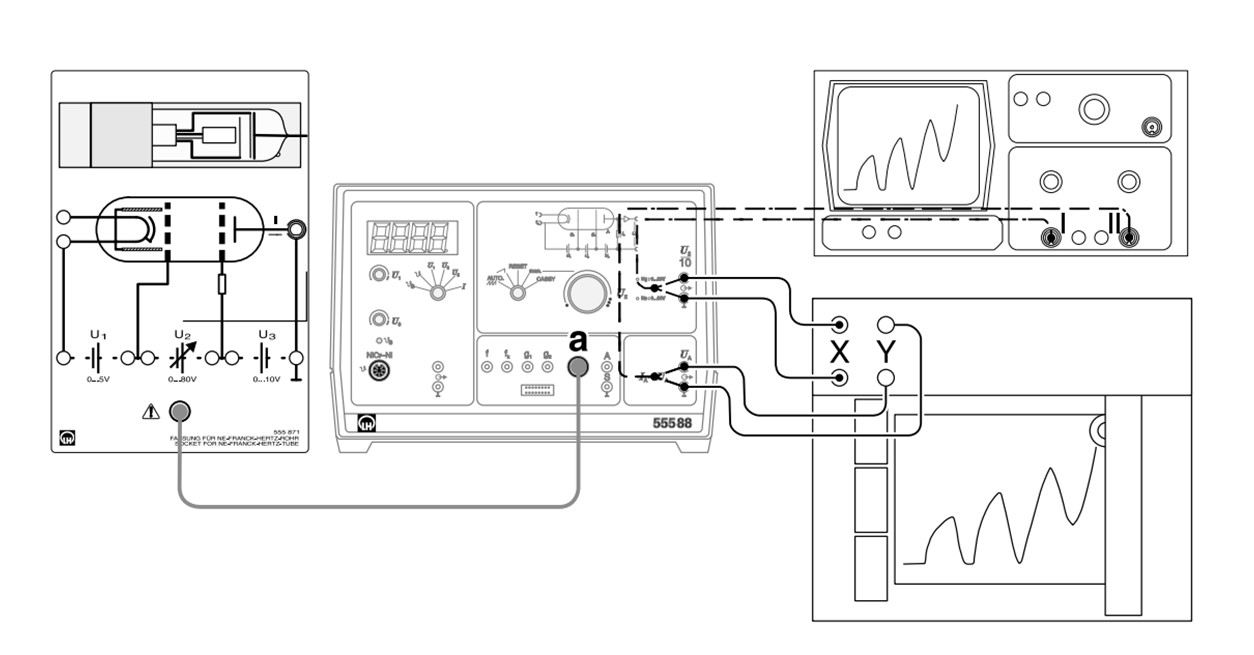
\includegraphics[width=5cm]{fig3.png}
		\caption{Experiment setup for Franck-Hertz experiment for neon.}
		\label{fig:3}
	\end{figure}

\subsection{Carrying out the experiment}

\subsubsection{Franck-Hertz curve:}
	\begin{enumerate}[label=\arabic*.]
		\item Record the Franck-Hertz curve (see preliminary remark). 
	\end{enumerate}

\subsubsection{Light emission:}
	\begin{enumerate}[label=\arabic*.]
		\item Set the operating mode switch to MAN. 
		\item Optimize the acceleration voltage U2 until you can clearly see a red-yellow luminance zone between grids G1 and G2. 
		\item Additionally, find the optimum acceleration voltages for two or three luminance zones and log these values. 
	\end{enumerate}

\subsection{Measuring example and evaluation}

\subsubsection{Franck-Hertz curve:}
	U1 = 2.06 V, U3 = 7.94 V 

	The distance between the vertical lines (these were placed by eye on the main points of the maxima) has an average value of DU2 = 18.5 V. This value is much closer to the excitation energies for the 3p-levels of neon (18.4 – 19.0 eV) than to the energies of the 3s-levels (16.6 – 16.9 eV). Thus, the probability of excitation to the latter due to inelastic electron collision is significantly less. The substructure in the measured curve shows that the excitation of the 3s-levels cannot be ignored altogether. Note that for double and multiple collisions, each combination of excitation of a 3s-level and a 3p-level occurs. 

\subsubsection{Light emission:}
	U1 = 2.06 V, U3 = 7.94 V 

	The luminance layers are zones of high excitation density. They can be compared directly with the minima of the FranckHertz curve. Their spacing corresponds to an acceleration voltage U2 = 19 V. Therefore, an additional luminance layer is generated each time U2 is increased by approx. 19 V 

	\begin{figure}[htb!]
		\centering
		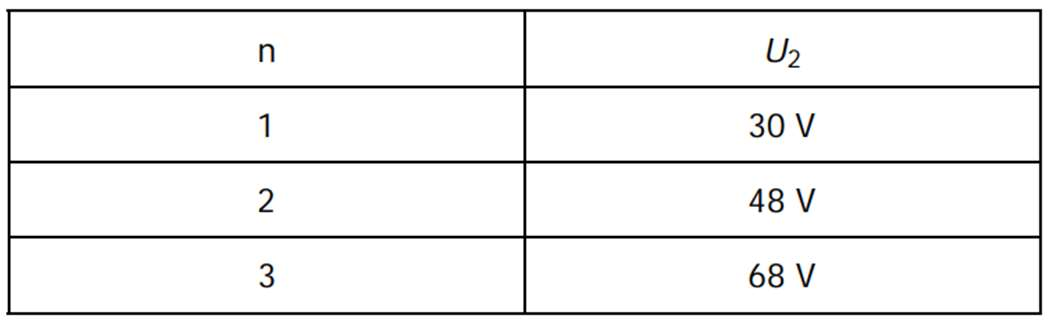
\includegraphics[width=5cm]{fig4.png}
		\caption{}
		\label{fig:4}
	\end{figure}

	\begin{figure}[htb!]
		\centering
		\includegraphics[width=5cm]{fig5.jpg}
		\caption{}
		\label{fig:5}
	\end{figure}

%----------------------------------------------------------------------------------------
%	RESULT AND DISCUSSION
%----------------------------------------------------------------------------------------

\section{Result and Discussion}

\subsection{Franck-Hertz curve:}
	\begin{figure}[htb!]
		\centering
		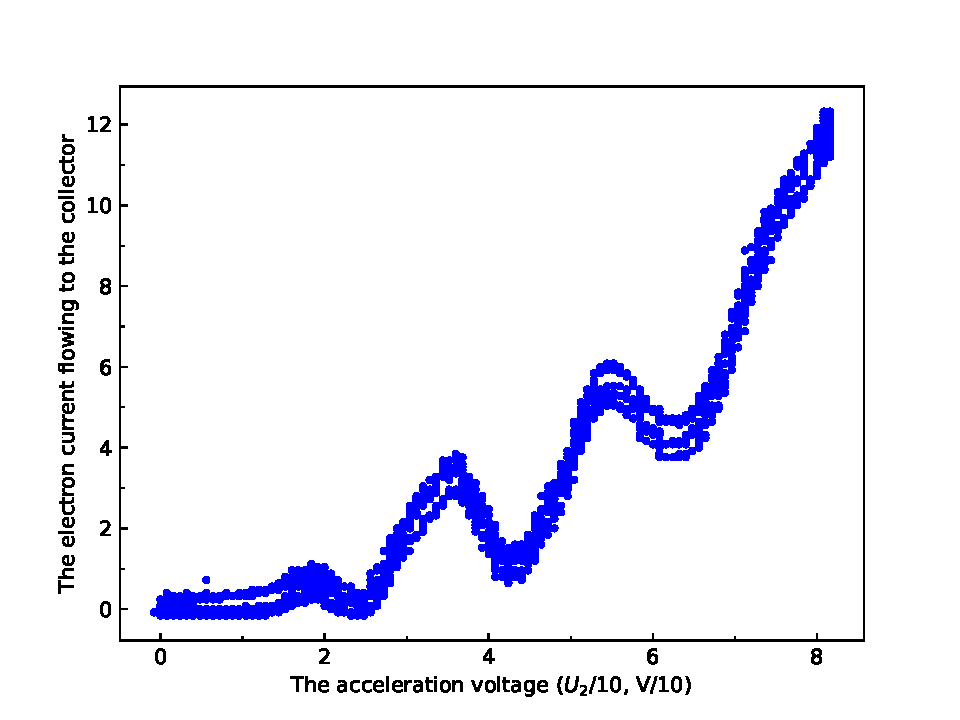
\includegraphics[width=8cm]{fig6.pdf}
		\caption{Data fitting for Franck-Hertz curve.}
		\label{fig:6}
	\end{figure}

	Fig. 6은 0 V부터 80 V까지 $U_2$를 조절하여 전하의 흐름 데이터를 fitting한 것이다. 그래프를 분석하여 Tab. 1으로 정리한 것이다.

	\begin{table}[htb!]
		\label{tab:1}
		\centering
		\caption{전하의 흐름이 상승(peak)하는 부분이다.}
		\begin{tabular}{c|c}
				\noalign{\smallskip}\noalign{\smallskip}\hline\hline
				$n$ & $U_2$ (V) \\
			\hline
				1 & 19 \\
				2 & 36 \\
				3 & 55 \\
			\hline
			\hline
		\end{tabular}
	\end{table}

	이론적인 부분과 비교했을 때, 실 데이터와 약 30\% 차이가 나지만 그 간격과 그래프 모양을 보면 차이가 많지 않음을 볼 수 있다.

\subsubsection{Light emission:}
	\begin{figure}[htb!]
		\centering
		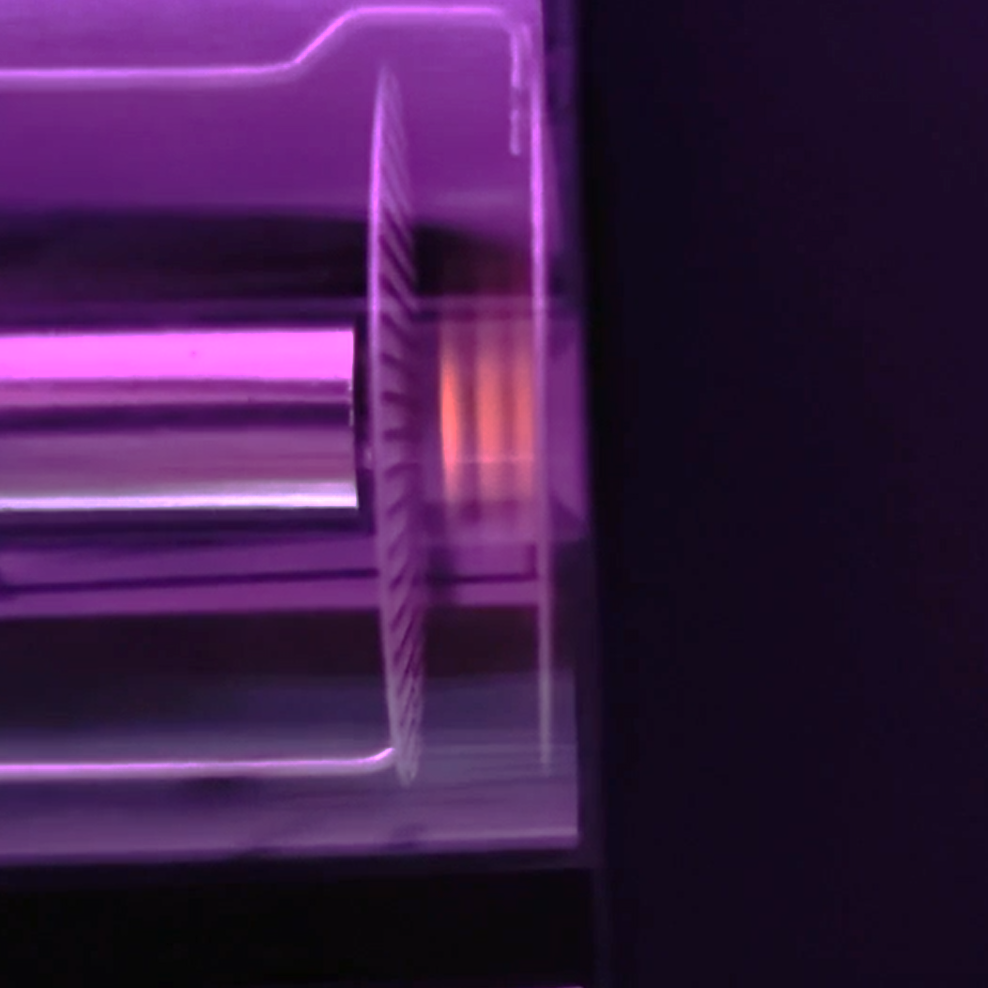
\includegraphics[width=5cm]{fig7.1.png}
		\caption{Light emission}
		\label{fig:7}
	\end{figure}

	\begin{table}[htb!]
		\label{tab:2}
		\centering
		\caption{전하의 흐름이 상승(peak)하는 부분이다.}
		\resizebox{\textwidth}{!}{
		\begin{tabular*}{\textwidth}{lll|@{\extracolsep{\fill}}ll}
				\noalign{\smallskip}\noalign{\smallskip}\hline\hline
				& $n$ & & $U_2$ (V) & \\
			\hline
				& 1 & & 29.9 & \\
				& 2 & & 47.4 & \\
				& 3 & & 65.7 & \\
			\hline
			\hline
		\end{tabular*}
		}
	\end{table}

	이론적인 부분과 비교했을 때, 오차가 1\% 내이기에 이론값과 차이가 없음을 알 수 있다.

%----------------------------------------------------------------------------------------
%	CONCLUSIONS
%----------------------------------------------------------------------------------------

\section{Conclusions}

	Franck-Hertz experiment with neon에서 네온 원자에 속박된 전자가 양자화되어 있음을 확인할 수 있었다. 특히 Fig. 6을 보면 특정 peak에서 전류가 상승하는 것을 볼 수 있고, 이는 전하가 이동함을 뜻한다. 즉, 그 순간에 속박에서 풀려난다는 것을 알 수 있다. 또한, Fig. 7을 통해 orbit을 건널 때마다 에너지, 즉 빛이 방출됨을 볼 수 있었다.

%----------------------------------------------------------------------------------------
%	FITTING CODE FOR PYTHON
%----------------------------------------------------------------------------------------

\section{Fitting code for Python}

\begin{figure*}[htb!]
	\centering
	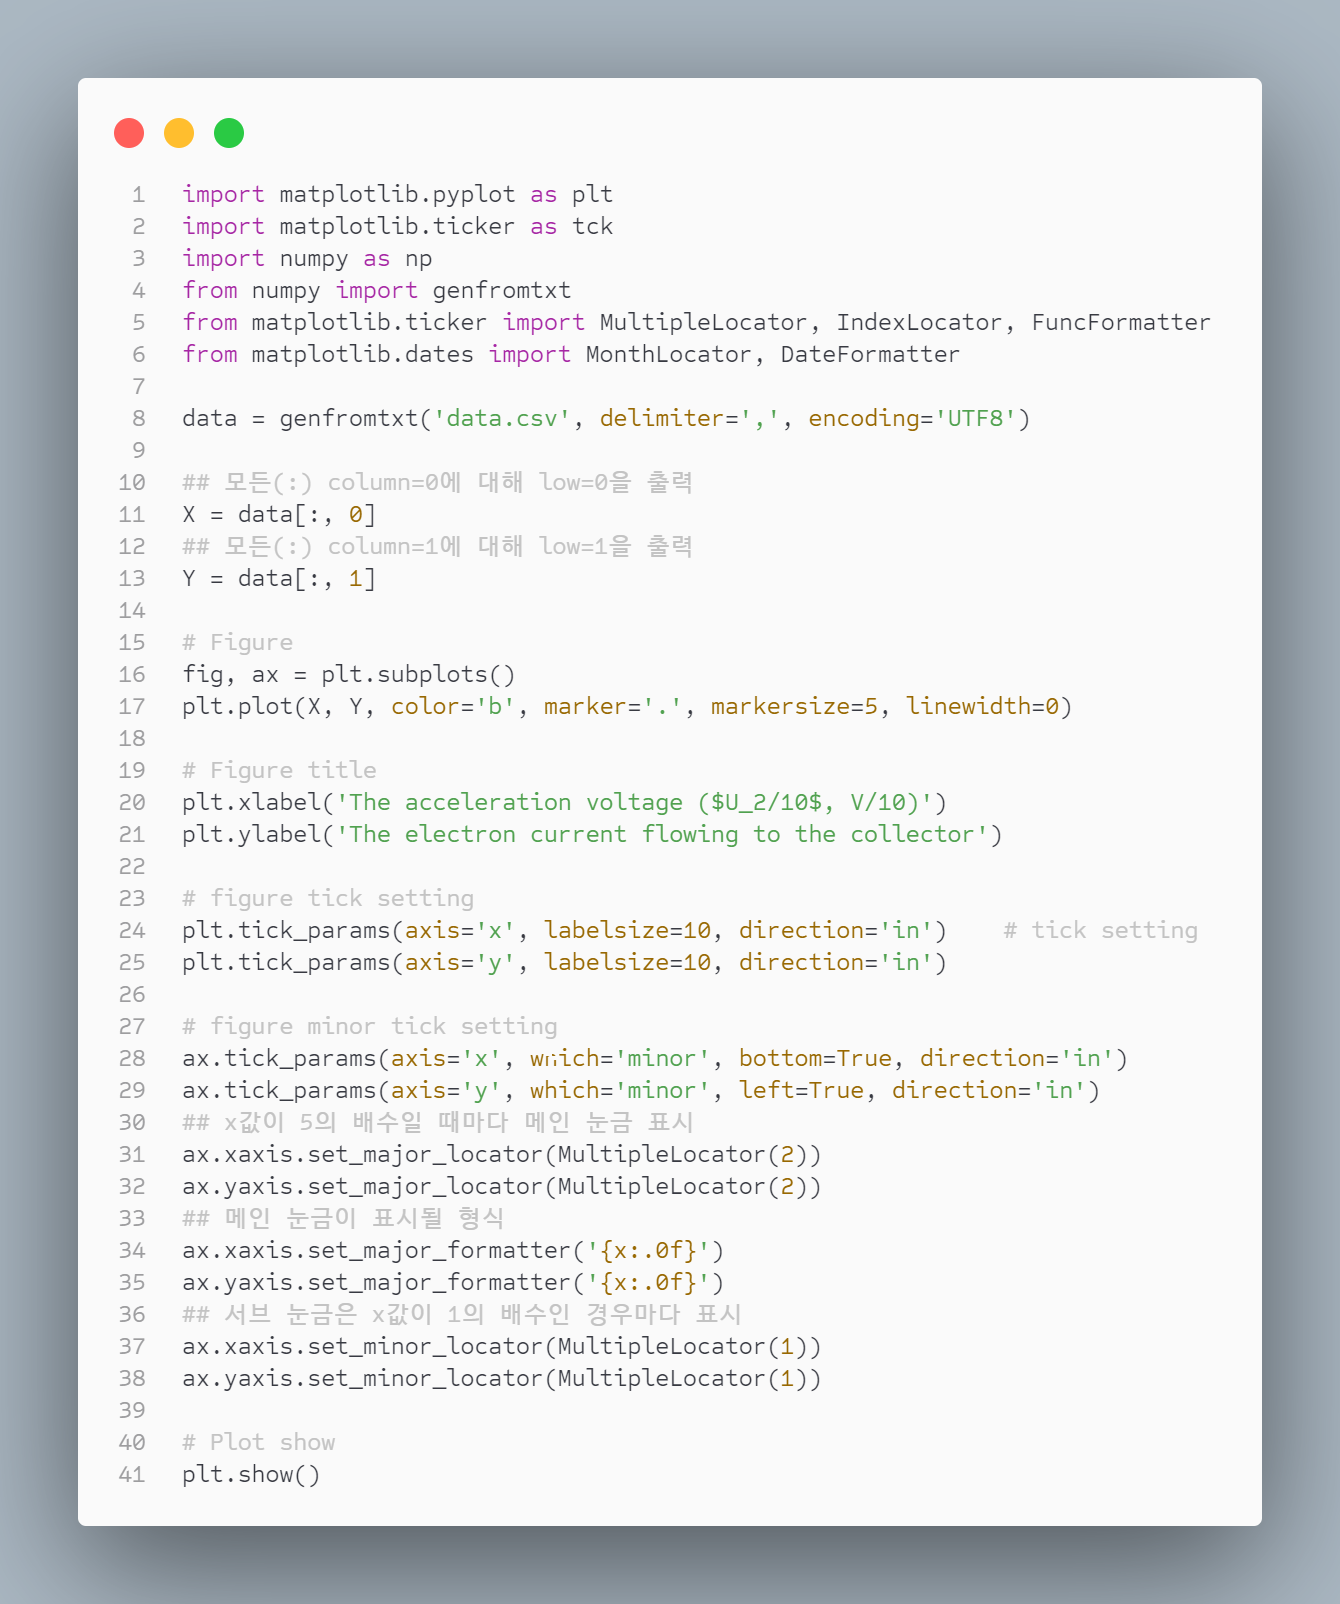
\includegraphics[width=8cm]{code1.png}
	\label{fig:code}
\end{figure*}

%----------------------------------------------------------------------------------------
%	BIBLIOGRAPHY
%----------------------------------------------------------------------------------------

% \printbibliography % Output the bibliography

%----------------------------------------------------------------------------------------

\end{document}